\documentclass[aspectratio=169,12pt]{beamer}

% Theme and colors
\usetheme{Madrid}
\usecolortheme{whale}
\setbeamertemplate{navigation symbols}{}
\setbeamertemplate{footline}[frame number]

% Packages
\usepackage{amsmath,amssymb,amsthm}
\usepackage{graphicx}
\usepackage{tikz}
\usetikzlibrary{trees,shapes,arrows,positioning,calc}
\usepackage{booktabs}
\usepackage{array}
\usepackage{multirow}
\usepackage{algorithm}
\usepackage{algorithmic}
\usepackage{xcolor}
\usepackage{hyperref}

% Custom colors
\definecolor{codegreen}{rgb}{0,0.6,0}
\definecolor{codepurple}{rgb}{0.58,0,0.82}
\definecolor{darkblue}{rgb}{0,0,0.7}

% Title information
\title[Shannon-Fano Coding]{Shannon-Fano Coding}
\subtitle{A Foundation of Data Compression}
\author[Mahesh C]{\textbf{Mahesh C}\\FISAT}
\institute{Federal Institute of Science and Technology (FISAT)\\Multimedia Technology Class}
\date{\today}

\begin{document}

% Title slide
\begin{frame}
    \titlepage
\end{frame}

% Outline
\begin{frame}{Outline}
    \tableofcontents
\end{frame}

%==============================================================================
\section{What is Coding?}
%==============================================================================

\begin{frame}{Can You Decode This Message?}
    \begin{center}
        \Huge{\textcolor{darkblue}{\textbf{XFMDPNF UP GJTBU}}}
    \end{center}
    
    \vspace{1cm}
    \begin{center}
        \Large{\textit{What does this say?}}
        
        \vspace{0.5cm}
        \textbf{Take 30 seconds to guess...}
    \end{center}
    
    \vspace{1cm}
    \begin{center}
        \begin{tabular}{|c|c|c|c|c|c|c|c|c|c|c|c|c|c|c|c|}
            \hline
            X & F & M & D & P & N & F & & U & P & & G & J & T & B & U \\
            \hline
            $\downarrow$ & $\downarrow$ & $\downarrow$ & $\downarrow$ & $\downarrow$ & $\downarrow$ & $\downarrow$ & & $\downarrow$ & $\downarrow$ & & $\downarrow$ & $\downarrow$ & $\downarrow$ & $\downarrow$ & $\downarrow$ \\
            \hline
            ? & ? & ? & ? & ? & ? & ? & & ? & ? & & ? & ? & ? & ? & ? \\
            \hline
        \end{tabular}
    \end{center}
\end{frame}

\begin{frame}{Here's a Hint...}
    \begin{center}
        \Large{\textcolor{darkblue}{\textbf{XFMDPNF UP GJTBU}}}
    \end{center}
    
    \vspace{0.5cm}
    \begin{block}{Hint}
        Each letter has been \textbf{shifted forward by 1 position} in the alphabet.
        
        A $\rightarrow$ B, \quad B $\rightarrow$ C, \quad C $\rightarrow$ D, \quad ... \quad Z $\rightarrow$ A
    \end{block}
    
    \vspace{0.5cm}
    \textbf{Now try again!}
    \begin{center}
        \begin{tabular}{|c|c|c|c|c|c|c|c|c|c|c|c|c|c|c|c|}
            \hline
            X & F & M & D & P & N & F & & U & P & & G & J & T & B & U \\
            \hline
            $\downarrow$ & $\downarrow$ & $\downarrow$ & $\downarrow$ & $\downarrow$ & $\downarrow$ & $\downarrow$ & & $\downarrow$ & $\downarrow$ & & $\downarrow$ & $\downarrow$ & $\downarrow$ & $\downarrow$ & $\downarrow$ \\
            \hline
            W & E & L & C & O & M & E & & T & O & & F & I & S & A & T \\
            \hline
        \end{tabular}
    \end{center}
    
    \vspace{0.5cm}
    \pause
    \begin{alertblock}{The Answer is...}
        \Huge{\textbf{WELCOME TO FISAT!}}
    \end{alertblock}
\end{frame}

\begin{frame}{Surprise --- That Was Coding!}
    \begin{alertblock}{What You Just Did}
        You performed \textbf{DECODING} --- converting coded information back to its original form!
    \end{alertblock}
    
    \vspace{0.3cm}
    \begin{columns}
        \begin{column}{0.5\textwidth}
            \textbf{Encoding (Sender):}
            \begin{center}
                WELCOME TO FISAT
                
                $\downarrow$ \textit{Shift +1}
                
                XFMDPNF UP GJTBU
            \end{center}
        \end{column}
        \begin{column}{0.5\textwidth}
            \textbf{Decoding (Receiver):}
            \begin{center}
                XFMDPNF UP GJTBU
                
                $\downarrow$ \textit{Shift -1}
                
                WELCOME TO FISAT
            \end{center}
        \end{column}
    \end{columns}
    
    \vspace{0.5cm}
    \begin{block}{This is called Caesar Cipher}
        Used by Julius Caesar 2000+ years ago to send secret military messages!
        
        \textbf{Code = Rule to transform information}
    \end{block}
    
    \vspace{0.3cm}
    \textit{Today we'll learn a different type of coding --- not for secrecy, but for \textbf{efficiency}!}
\end{frame}

\begin{frame}{What is ``Coding'' in Information Theory?}
    \begin{alertblock}{Important Clarification}
        \textbf{Coding} here does NOT mean programming or writing software!
    \end{alertblock}
    
    \vspace{0.3cm}
    \begin{block}{Definition}
        \textbf{Coding} = Converting information from one representation to another
    \end{block}
    
    \vspace{0.3cm}
    \textbf{You already use coding every day!}
    \begin{itemize}
        \item \textbf{Language:} Thoughts $\rightarrow$ Words $\rightarrow$ Speech sounds
        \item \textbf{Writing:} Words $\rightarrow$ Letters on paper
        \item \textbf{Emojis:} Emotions $\rightarrow$ Smiley, Party, Heart symbols
        \item \textbf{Traffic lights:} Instructions $\rightarrow$ Red/Yellow/Green
        \item \textbf{Music:} Sound $\rightarrow$ Notes on a sheet (Do Re Mi...)
    \end{itemize}
\end{frame}

\begin{frame}{Everyday Examples of Codes}
    \begin{columns}
        \begin{column}{0.5\textwidth}
            \textbf{1. Morse Code (1840s)}
            \begin{center}
                \begin{tabular}{c|c}
                    \toprule
                    Letter & Code \\
                    \midrule
                    A & $\cdot -$ \\
                    B & $- \cdot \cdot \cdot$ \\
                    E & $\cdot$ \\
                    S & $\cdot \cdot \cdot$ \\
                    O & $- - -$ \\
                    \bottomrule
                \end{tabular}
            \end{center}
            \textbf{SOS} = $\cdot\cdot\cdot$ $---$ $\cdot\cdot\cdot$
            
            \vspace{0.3cm}
            \textit{Notice: 'E' (common) is short!}
        \end{column}
        \begin{column}{0.5\textwidth}
            \textbf{2. Braille (for visually impaired)}
            \begin{itemize}
                \item Each letter = pattern of 6 dots
                \item Converts visual text to touch
            \end{itemize}
            
            \vspace{0.3cm}
            \textbf{3. Binary Code (Computers)}
            \begin{itemize}
                \item A = 01000001
                \item B = 01000010
                \item Everything is 0s and 1s!
            \end{itemize}
        \end{column}
    \end{columns}
\end{frame}

\begin{frame}{Why Do We Need Different Codes?}
    \textbf{Different situations need different codes:}
    
    \vspace{0.5cm}
    \begin{columns}
        \begin{column}{0.5\textwidth}
            \textbf{Telegram (pay per character):}
            \begin{itemize}
                \item ``ARRIVING TOMORROW MORNING''
                \item Shorter = Cheaper!
                \item People invented abbreviations
            \end{itemize}
            
            \vspace{0.3cm}
            \textbf{SMS (160 character limit):}
            \begin{itemize}
                \item ``c u l8r'' instead of ``see you later''
                \item Shorter codes for common phrases
            \end{itemize}
        \end{column}
        \begin{column}{0.5\textwidth}
            \textbf{PIN Codes in India:}
            \begin{itemize}
                \item 6 digits represent location
                \item 682030 = Specific area in Kochi
                \item Compact way to encode address
            \end{itemize}
            
            \vspace{0.3cm}
            \textbf{Vehicle Registration:}
            \begin{itemize}
                \item KL-07-AB-1234
                \item State + District + Series + Number
                \item Structured code for identification
            \end{itemize}
        \end{column}
    \end{columns}
\end{frame}

\begin{frame}{The Key Question: What Makes a Good Code?}
    \begin{center}
        \Large{\textbf{If you could design your own code, how would you do it?}}
    \end{center}
    
    \vspace{0.5cm}
    \textbf{Properties of a good code:}
    \begin{enumerate}
        \item \textbf{Efficient:} Uses minimum symbols/bits
        \item \textbf{Unambiguous:} Each message has only one meaning
        \item \textbf{Decodable:} Can recover original message perfectly
    \end{enumerate}
    
    \vspace{0.5cm}
    \begin{block}{The Smart Idea}
        \textbf{Frequently used items} $\rightarrow$ \textbf{Short codes}
        
        \textbf{Rarely used items} $\rightarrow$ \textbf{Long codes}
        
        \vspace{0.2cm}
        This is exactly what \textbf{Shannon-Fano Coding} does!
    \end{block}
\end{frame}

\begin{frame}{From Codes to Computers: Binary World}
    \textbf{Computers only understand 0 and 1 (Binary)}
    
    \vspace{0.3cm}
    \begin{columns}
        \begin{column}{0.5\textwidth}
            \textbf{Why binary?}
            \begin{itemize}
                \item Electronic switches: ON (1) or OFF (0)
                \item Simple and reliable
                \item Easy to store and transmit
            \end{itemize}
            
            \vspace{0.3cm}
            \textbf{Everything becomes binary:}
            \begin{itemize}
                \item Text $\rightarrow$ Binary
                \item Images $\rightarrow$ Binary
                \item Audio $\rightarrow$ Binary
                \item Video $\rightarrow$ Binary
            \end{itemize}
        \end{column}
        \begin{column}{0.5\textwidth}
            \textbf{Standard ASCII Code:}
            \begin{center}
                \begin{tabular}{c|c}
                    \toprule
                    Character & Binary (8 bits) \\
                    \midrule
                    A & 01000001 \\
                    B & 01000010 \\
                    a & 01100001 \\
                    0 & 00110000 \\
                    Space & 00100000 \\
                    \bottomrule
                \end{tabular}
            \end{center}
            
            \vspace{0.2cm}
            \textit{Every character = 8 bits (fixed)}
            
            \textit{Is this efficient? (Think about it!)}
        \end{column}
    \end{columns}
\end{frame}

\begin{frame}{The Problem with Fixed-Length Codes}
    \textbf{ASCII uses 8 bits for EVERY character:}
    
    \vspace{0.3cm}
    \begin{columns}
        \begin{column}{0.5\textwidth}
            \textbf{``HELLO'' in ASCII:}
            \begin{itemize}
                \item H = 01001000
                \item E = 01000101
                \item L = 01001100
                \item L = 01001100
                \item O = 01001111
            \end{itemize}
            Total: $5 \times 8 = 40$ bits
        \end{column}
        \begin{column}{0.5\textwidth}
            \textbf{But wait...}
            \begin{itemize}
                \item 'E' is the most common letter
                \item 'Z' is very rare
                \item Both use 8 bits! (Wasteful!)
            \end{itemize}
            
            \vspace{0.3cm}
            \textbf{Better idea:}
            \begin{itemize}
                \item Give 'E' a short code (2-3 bits)
                \item Give 'Z' a longer code
                \item Average bits per letter drops!
            \end{itemize}
        \end{column}
    \end{columns}
    
    \vspace{0.5cm}
    \begin{block}{This is Variable-Length Coding!}
        Shannon-Fano coding assigns \textbf{different length codes} based on \textbf{how often} each symbol appears.
    \end{block}
\end{frame}

%==============================================================================
\section{Introduction to Data Compression}
%==============================================================================

\begin{frame}{Why Data Compression?}
    \begin{columns}
        \begin{column}{0.6\textwidth}
            \textbf{The Need for Compression:}
            \begin{itemize}
                \item Limited storage capacity
                \item Limited bandwidth for transmission
                \item Cost reduction
                \item Faster data transfer
            \end{itemize}
            \vspace{0.5cm}
            \textbf{Types of Compression:}
            \begin{itemize}
                \item \textcolor{darkblue}{Lossless} - Perfect reconstruction
                \item \textcolor{codepurple}{Lossy} - Approximate reconstruction
            \end{itemize}
        \end{column}
        \begin{column}{0.4\textwidth}
            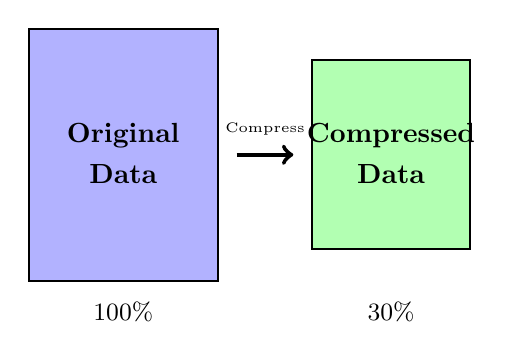
\begin{tikzpicture}[scale=0.8]
                \draw[fill=blue!30, thick] (0,0) rectangle (3,4);
                \node at (1.5,2.3) {\textbf{Original}};
                \node at (1.5,1.7) {\textbf{Data}};
                \draw[->,ultra thick] (3.3,2) -- (4.2,2);
                \node[rotate=0] at (3.75,2.4) {\tiny Compress};
                \draw[fill=green!30, thick] (4.5,0.5) rectangle (7,3.5);
                \node at (5.75,2.3) {\textbf{Compressed}};
                \node at (5.75,1.7) {\textbf{Data}};
                \node at (1.5,-0.5) {\small 100\%};
                \node at (5.75,-0.5) {\small 30\%};
            \end{tikzpicture}
        \end{column}
    \end{columns}
\end{frame}

\begin{frame}{Real-World Example: Why Compression Matters}
    \textbf{Scenario: Sending a 4K Movie over the Internet}
    
    \begin{columns}
        \begin{column}{0.5\textwidth}
            \textbf{Without Compression:}
            \begin{itemize}
                \item Raw 4K video: $\sim$500 GB for 2-hour movie
                \item On 50 Mbps connection: $\sim$22 hours to download!
                \item Netflix monthly data: $\sim$15 TB per user
            \end{itemize}
        \end{column}
        \begin{column}{0.5\textwidth}
            \textbf{With Compression (H.265):}
            \begin{itemize}
                \item Compressed: $\sim$8-15 GB
                \item Download time: $\sim$30-45 minutes
                \item 97\% storage saved!
            \end{itemize}
        \end{column}
    \end{columns}
    
    \vspace{0.5cm}
    \begin{alertblock}{Daily Life Examples}
        \begin{itemize}
            \item \textbf{WhatsApp:} Compresses photos from 5MB to 100KB before sending
            \item \textbf{Spotify:} Streams 320kbps instead of 1411kbps (CD quality)
            \item \textbf{ZIP files:} Reduces document folder by 70-90\%
        \end{itemize}
    \end{alertblock}
\end{frame}

\begin{frame}{Information Theory Basics}
    \textbf{Claude Shannon (1948)} - Father of Information Theory
    
    \vspace{0.3cm}
    \begin{block}{Key Insight}
        The amount of information in a message is related to its \textbf{probability}.
        Rare events carry more information than common events.
    \end{block}
    
    \vspace{0.3cm}
    \textbf{Self-Information} of an event with probability $p$:
    \begin{equation}
        I(x) = -\log_2 p(x) = \log_2 \frac{1}{p(x)} \quad \text{(bits)}
    \end{equation}
    
    \vspace{0.3cm}
    \textbf{Example:}
    \begin{itemize}
        \item If $p = 0.5$: $I = -\log_2(0.5) = 1$ bit
        \item If $p = 0.25$: $I = -\log_2(0.25) = 2$ bits
        \item If $p = 0.125$: $I = -\log_2(0.125) = 3$ bits
    \end{itemize}
\end{frame}

\begin{frame}{Entropy - Average Information}
    \begin{block}{Shannon Entropy}
        The \textbf{entropy} $H(X)$ of a discrete random variable $X$ with possible values $\{x_1, x_2, \ldots, x_n\}$ and probability mass function $P(X)$:
        \begin{equation}
            \boxed{H(X) = -\sum_{i=1}^{n} p(x_i) \log_2 p(x_i) = \sum_{i=1}^{n} p(x_i) \log_2 \frac{1}{p(x_i)}}
        \end{equation}
    \end{block}
    
    \vspace{0.3cm}
    \textbf{Properties of Entropy:}
    \begin{itemize}
        \item $H(X) \geq 0$ (always non-negative)
        \item $H(X) = 0$ if and only if one outcome has probability 1
        \item $H(X)$ is maximum when all outcomes are equally likely
        \item Maximum entropy: $H_{max} = \log_2 n$
    \end{itemize}
\end{frame}

\begin{frame}{Entropy Calculation Example}
    \textbf{Example:} A source emits symbols $\{A, B, C, D\}$ with probabilities:
    
    \begin{center}
        \begin{tabular}{c|cccc}
            \toprule
            Symbol & A & B & C & D \\
            \midrule
            Probability & 0.5 & 0.25 & 0.125 & 0.125 \\
            \bottomrule
        \end{tabular}
    \end{center}
    
    \vspace{0.3cm}
    \textbf{Entropy Calculation:}
    \begin{align*}
        H(X) &= -[0.5 \log_2(0.5) + 0.25 \log_2(0.25) \\
             &\quad + 0.125 \log_2(0.125) + 0.125 \log_2(0.125)] \\
        &= -[0.5(-1) + 0.25(-2) + 0.125(-3) + 0.125(-3)] \\
        &= 0.5 + 0.5 + 0.375 + 0.375 \\
        &= \boxed{1.75 \text{ bits/symbol}}
    \end{align*}
\end{frame}

\begin{frame}{Real-World Entropy Example: English Text}
    \textbf{Letter Frequencies in English:}
    
    \begin{columns}
        \begin{column}{0.5\textwidth}
            \begin{center}
                \begin{tabular}{c|c}
                    \toprule
                    Letter & Frequency \\
                    \midrule
                    E & 12.7\% \\
                    T & 9.1\% \\
                    A & 8.2\% \\
                    O & 7.5\% \\
                    I & 7.0\% \\
                    N & 6.7\% \\
                    S & 6.3\% \\
                    ... & ... \\
                    Z & 0.07\% \\
                    \bottomrule
                \end{tabular}
            \end{center}
        \end{column}
        \begin{column}{0.5\textwidth}
            \textbf{Key Insight:}
            \begin{itemize}
                \item 'E' appears 180x more than 'Z'
                \item Fixed 8-bit ASCII wastes bits!
                \item Entropy of English $\approx$ 4.2 bits/letter
                \item Potential savings: 48\%!
            \end{itemize}
            
            \vspace{0.3cm}
            \textbf{Shannon-Fano Idea:}
            \begin{itemize}
                \item Give 'E' a short code (2-3 bits)
                \item Give 'Z' a long code (8+ bits)
                \item Average code length drops!
            \end{itemize}
        \end{column}
    \end{columns}
\end{frame}

%==============================================================================
\section{Shannon-Fano Coding Fundamentals}
%==============================================================================

\begin{frame}{Simple Analogy: Weather Reporting}
    \textbf{Imagine you're a weather reporter in Kerala:}
    
    \begin{columns}
        \begin{column}{0.5\textwidth}
            \textbf{Weather Probabilities:}
            \begin{center}
                \begin{tabular}{l|c}
                    \toprule
                    Weather & Probability \\
                    \midrule
                    Sunny & 50\% \\
                    Cloudy & 25\% \\
                    Rainy & 15\% \\
                    Stormy & 10\% \\
                    \bottomrule
                \end{tabular}
            \end{center}
        \end{column}
        \begin{column}{0.5\textwidth}
            \textbf{Efficient Codes:}
            \begin{center}
                \begin{tabular}{l|c}
                    \toprule
                    Weather & Code \\
                    \midrule
                    Sunny & 0 (1 bit) \\
                    Cloudy & 10 (2 bits) \\
                    Rainy & 110 (3 bits) \\
                    Stormy & 111 (3 bits) \\
                    \bottomrule
                \end{tabular}
            \end{center}
        \end{column}
    \end{columns}
    
    \vspace{0.5cm}
    \begin{block}{The Core Idea}
        \textbf{Common events $\rightarrow$ Short codes} | \textbf{Rare events $\rightarrow$ Long codes}
        
        Just like in Morse code: 'E' = $\cdot$ (1 symbol), 'Q' = $--\cdot-$ (4 symbols)
    \end{block}
\end{frame}

\begin{frame}{What is Shannon-Fano Coding?}
    \begin{block}{Definition}
        Shannon-Fano coding is a \textbf{prefix-free}, \textbf{variable-length} coding technique that assigns shorter codes to more frequent symbols.
    \end{block}
    
    \vspace{0.3cm}
    \textbf{Historical Background:}
    \begin{itemize}
        \item Developed independently by \textbf{Claude Shannon} and \textbf{Robert Fano} in 1948-1949
        \item One of the first practical entropy coding methods
        \item Precursor to Huffman coding
    \end{itemize}
    
    \vspace{0.3cm}
    \textbf{Key Properties:}
    \begin{itemize}
        \item \textcolor{codegreen}{Prefix-free code} - No codeword is a prefix of another
        \item Variable-length encoding based on symbol probability
        \item Instantaneously decodable
        \item Near-optimal but not always optimal
    \end{itemize}
\end{frame}

\begin{frame}{Prefix-Free Codes}
    \begin{columns}
        \begin{column}{0.5\textwidth}
            \textbf{Why Prefix-Free?}
            \begin{itemize}
                \item Allows \textbf{instantaneous decoding}
                \item No need for separators
                \item Unambiguous decoding
            \end{itemize}
            
            \vspace{0.5cm}
            \textbf{Example - NOT Prefix-Free:}
            \begin{center}
                \begin{tabular}{cc}
                    A $\rightarrow$ 0 & B $\rightarrow$ 01 \\
                \end{tabular}
            \end{center}
            Problem: Is ``01'' = ``AB'' or ``B''?
        \end{column}
        \begin{column}{0.5\textwidth}
            \textbf{Prefix-Free Example:}
            \begin{center}
                \begin{tabular}{cc}
                    A $\rightarrow$ 0 & B $\rightarrow$ 10 \\
                    C $\rightarrow$ 110 & D $\rightarrow$ 111 \\
                \end{tabular}
            \end{center}
            
            \vspace{0.3cm}
            Decode ``011010'':
            \begin{itemize}
                \item 0 $\rightarrow$ A
                \item 110 $\rightarrow$ C
                \item 10 $\rightarrow$ B
            \end{itemize}
            Result: \textbf{ACB}
        \end{column}
    \end{columns}
\end{frame}

%==============================================================================
\section{Shannon-Fano Algorithm}
%==============================================================================

\begin{frame}{The Shannon-Fano Algorithm}
    \begin{block}{Algorithm Steps}
        \begin{enumerate}
            \item \textbf{Sort} symbols in decreasing order of probability
            \item \textbf{Divide} the list into two groups with approximately equal total probabilities
            \item \textbf{Assign} `0' to the first group and `1' to the second group
            \item \textbf{Recursively} apply steps 2-3 to each group until each group contains only one symbol
        \end{enumerate}
    \end{block}
    
    \vspace{0.3cm}
    \textbf{Key Principle:} At each step, try to balance the probabilities on each side as equally as possible.
\end{frame}

\begin{frame}{Algorithm Pseudocode}
    \begin{algorithm}[H]
        \caption{Shannon-Fano Coding}
        \begin{algorithmic}[1]
            \STATE \textbf{Input:} List of symbols with probabilities
            \STATE \textbf{Output:} Binary codes for each symbol
            \STATE Sort symbols by probability (descending)
            \STATE Call ShannonFano(symbols, code = "")
            \STATE
            \STATE \textbf{Procedure} ShannonFano(symbols, code)
            \IF{length(symbols) == 1}
                \STATE Assign code to the symbol
            \ELSE
                \STATE Divide symbols into two groups (balanced probabilities)
                \STATE ShannonFano(group1, code + "0")
                \STATE ShannonFano(group2, code + "1")
            \ENDIF
        \end{algorithmic}
    \end{algorithm}
\end{frame}

\begin{frame}{Shannon-Fano: Detailed Example}
    \textbf{Given:} Source symbols with the following probabilities:
    
    \begin{center}
        \begin{tabular}{c|c}
            \toprule
            Symbol & Probability \\
            \midrule
            A & 0.35 \\
            B & 0.25 \\
            C & 0.20 \\
            D & 0.12 \\
            E & 0.08 \\
            \bottomrule
        \end{tabular}
    \end{center}
    
    \textbf{Step 1:} Already sorted in decreasing order of probability.
    
    \vspace{0.3cm}
    Total probability = 1.0 (verified)
\end{frame}

\begin{frame}{Example: First Division}
    \textbf{Step 2:} Divide into two groups with balanced probabilities
    
    \begin{center}
        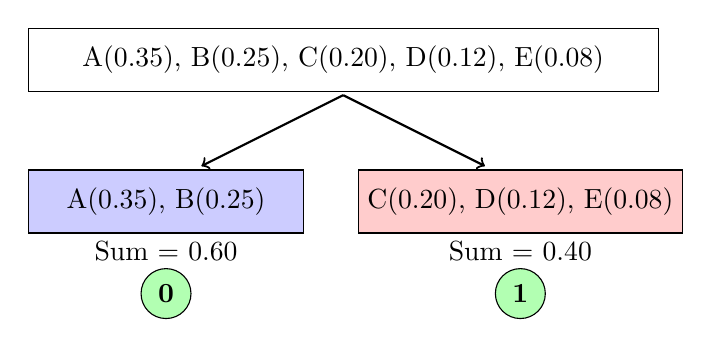
\begin{tikzpicture}[scale=0.9]
            % All symbols
            \node[draw, minimum width=8cm, minimum height=0.8cm] at (0,3) {A(0.35), B(0.25), C(0.20), D(0.12), E(0.08)};
            
            % Division line
            \draw[->,thick] (0,2.5) -- (-2,1.5);
            \draw[->,thick] (0,2.5) -- (2,1.5);
            
            % Group 1
            \node[draw, fill=blue!20, minimum width=3.5cm, minimum height=0.8cm] at (-2.5,1) {A(0.35), B(0.25)};
            \node at (-2.5,0.3) {Sum = 0.60};
            \node[circle, draw, fill=green!30] at (-2.5,-0.3) {\textbf{0}};
            
            % Group 2
            \node[draw, fill=red!20, minimum width=3.5cm, minimum height=0.8cm] at (2.5,1) {C(0.20), D(0.12), E(0.08)};
            \node at (2.5,0.3) {Sum = 0.40};
            \node[circle, draw, fill=green!30] at (2.5,-0.3) {\textbf{1}};
        \end{tikzpicture}
    \end{center}
    
    \vspace{0.3cm}
    \textbf{Division Options:}
    \begin{itemize}
        \item \{A\} vs \{B,C,D,E\}: 0.35 vs 0.65 $\rightarrow$ Difference = 0.30
        \item \{A,B\} vs \{C,D,E\}: 0.60 vs 0.40 $\rightarrow$ Difference = 0.20 \checkmark
    \end{itemize}
\end{frame}

\begin{frame}{Example: Second Level Division}
    \textbf{Step 3:} Recursively divide each group
    
    \begin{center}
        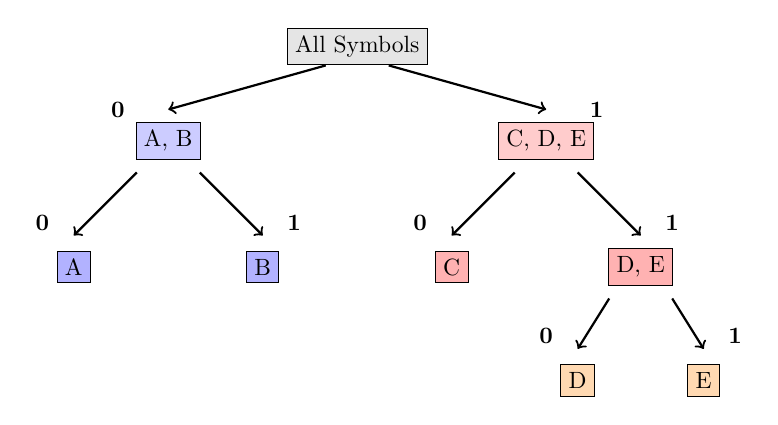
\begin{tikzpicture}[scale=0.8, every node/.style={scale=0.85}]
            % Root
            \node[draw, fill=gray!20] at (0,4) {All Symbols};
            
            % Level 1
            \draw[->,thick] (-0.5,3.7) -- (-3,3);
            \draw[->,thick] (0.5,3.7) -- (3,3);
            
            \node[draw, fill=blue!20] at (-3,2.5) {A, B};
            \node at (-3.8,3) {\textbf{0}};
            
            \node[draw, fill=red!20] at (3,2.5) {C, D, E};
            \node at (3.8,3) {\textbf{1}};
            
            % Level 2 - Left
            \draw[->,thick] (-3.5,2) -- (-4.5,1);
            \draw[->,thick] (-2.5,2) -- (-1.5,1);
            
            \node[draw, fill=blue!30] at (-4.5,0.5) {A};
            \node at (-5,1.2) {\textbf{0}};
            
            \node[draw, fill=blue!30] at (-1.5,0.5) {B};
            \node at (-1,1.2) {\textbf{1}};
            
            % Level 2 - Right
            \draw[->,thick] (2.5,2) -- (1.5,1);
            \draw[->,thick] (3.5,2) -- (4.5,1);
            
            \node[draw, fill=red!30] at (1.5,0.5) {C};
            \node at (1,1.2) {\textbf{0}};
            
            \node[draw, fill=red!30] at (4.5,0.5) {D, E};
            \node at (5,1.2) {\textbf{1}};
            
            % Level 3 - Right-Right
            \draw[->,thick] (4,0) -- (3.5,-0.8);
            \draw[->,thick] (5,0) -- (5.5,-0.8);
            
            \node[draw, fill=orange!30] at (3.5,-1.3) {D};
            \node at (3,-0.6) {\textbf{0}};
            
            \node[draw, fill=orange!30] at (5.5,-1.3) {E};
            \node at (6,-0.6) {\textbf{1}};
        \end{tikzpicture}
    \end{center}
\end{frame}

\begin{frame}{Example: Final Code Assignment}
    \textbf{Reading codes from root to leaves:}
    
    \begin{center}
        \begin{tabular}{c|c|c|c}
            \toprule
            Symbol & Probability & Code & Code Length \\
            \midrule
            A & 0.35 & 00 & 2 \\
            B & 0.25 & 01 & 2 \\
            C & 0.20 & 10 & 2 \\
            D & 0.12 & 110 & 3 \\
            E & 0.08 & 111 & 3 \\
            \bottomrule
        \end{tabular}
    \end{center}
    
    \vspace{0.5cm}
    \textbf{Verify Prefix-Free Property:}
    \begin{itemize}
        \item No code is a prefix of another \checkmark
        \item Uniquely decodable \checkmark
    \end{itemize}
\end{frame}

%==============================================================================
\section{Performance Analysis}
%==============================================================================

\begin{frame}{Average Code Length}
    \begin{block}{Average Code Length Formula}
        \begin{equation}
            L_{avg} = \sum_{i=1}^{n} p_i \cdot l_i
        \end{equation}
        where $p_i$ is the probability and $l_i$ is the code length of symbol $i$.
    \end{block}
    
    \vspace{0.3cm}
    \textbf{For our example:}
    \begin{align*}
        L_{avg} &= 0.35 \times 2 + 0.25 \times 2 + 0.20 \times 2 + 0.12 \times 3 + 0.08 \times 3 \\
        &= 0.70 + 0.50 + 0.40 + 0.36 + 0.24 \\
        &= \boxed{2.20 \text{ bits/symbol}}
    \end{align*}
\end{frame}

\begin{frame}{Entropy Comparison}
    \textbf{Calculate the entropy:}
    \begin{align*}
        H(X) &= -\sum_{i=1}^{n} p_i \log_2 p_i \\
        &= -(0.35 \log_2 0.35 + 0.25 \log_2 0.25 + 0.20 \log_2 0.20 \\
        &\quad + 0.12 \log_2 0.12 + 0.08 \log_2 0.08) \\
        &= -(0.35 \times (-1.514) + 0.25 \times (-2) + 0.20 \times (-2.322) \\
        &\quad + 0.12 \times (-3.059) + 0.08 \times (-3.644)) \\
        &= 0.530 + 0.500 + 0.464 + 0.367 + 0.292 \\
        &= \boxed{2.153 \text{ bits/symbol}}
    \end{align*}
\end{frame}

\begin{frame}{Coding Efficiency}
    \begin{block}{Efficiency Formula}
        \begin{equation}
            \eta = \frac{H(X)}{L_{avg}} \times 100\%
        \end{equation}
    \end{block}
    
    \vspace{0.3cm}
    \textbf{For our example:}
    \begin{equation*}
        \eta = \frac{2.153}{2.20} \times 100\% = \boxed{97.86\%}
    \end{equation*}
    
    \vspace{0.5cm}
    \begin{block}{Shannon's Source Coding Theorem}
        The average code length satisfies:
        \begin{equation}
            H(X) \leq L_{avg} < H(X) + 1
        \end{equation}
        Verification: $2.153 \leq 2.20 < 3.153$ \checkmark
    \end{block}
\end{frame}

\begin{frame}{Redundancy}
    \begin{block}{Redundancy Formula}
        \begin{equation}
            R = L_{avg} - H(X)
        \end{equation}
    \end{block}
    
    \vspace{0.3cm}
    \textbf{For our example:}
    \begin{equation*}
        R = 2.20 - 2.153 = \boxed{0.047 \text{ bits/symbol}}
    \end{equation*}
    
    \vspace{0.5cm}
    \textbf{Interpretation:}
    \begin{itemize}
        \item Lower redundancy = better compression
        \item Shannon-Fano achieves near-optimal performance
        \item Huffman coding can achieve even lower redundancy
    \end{itemize}
\end{frame}

%==============================================================================
\section{Complete Worked Example}
%==============================================================================

\begin{frame}{Practice Problem}
    \textbf{Problem:} Construct Shannon-Fano codes for the following source:
    
    \begin{center}
        \begin{tabular}{c|c}
            \toprule
            Symbol & Probability \\
            \midrule
            S1 & 0.30 \\
            S2 & 0.25 \\
            S3 & 0.20 \\
            S4 & 0.15 \\
            S5 & 0.10 \\
            \bottomrule
        \end{tabular}
    \end{center}
    
    \vspace{0.3cm}
    \textbf{Tasks:}
    \begin{enumerate}
        \item Construct the Shannon-Fano code
        \item Calculate average code length
        \item Calculate entropy
        \item Determine efficiency
    \end{enumerate}
\end{frame}

\begin{frame}{Practice Problem: Solution Tree}
    \begin{center}
        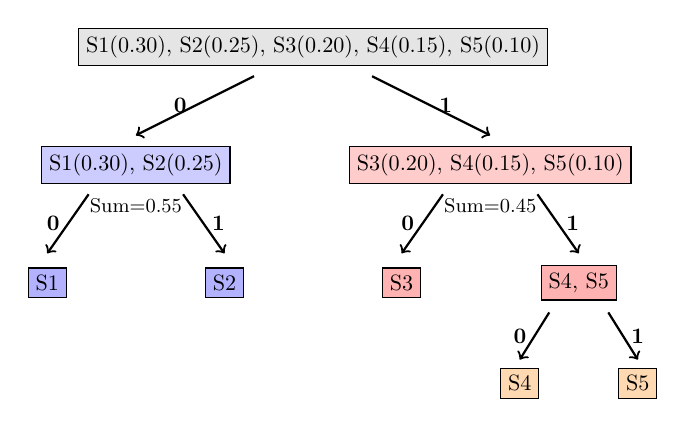
\begin{tikzpicture}[scale=0.75, every node/.style={scale=0.8}]
            % Level 0
            \node[draw, fill=gray!20, minimum width=6cm] at (0,5) {S1(0.30), S2(0.25), S3(0.20), S4(0.15), S5(0.10)};
            
            % Level 1
            \draw[->,thick] (-1,4.5) -- (-3,3.5) node[midway,left] {\textbf{0}};
            \draw[->,thick] (1,4.5) -- (3,3.5) node[midway,right] {\textbf{1}};
            
            \node[draw, fill=blue!20] at (-3,3) {S1(0.30), S2(0.25)};
            \node at (-3,2.3) {\small Sum=0.55};
            
            \node[draw, fill=red!20] at (3,3) {S3(0.20), S4(0.15), S5(0.10)};
            \node at (3,2.3) {\small Sum=0.45};
            
            % Level 2 - Left
            \draw[->,thick] (-3.8,2.5) -- (-4.5,1.5) node[midway,left] {\textbf{0}};
            \draw[->,thick] (-2.2,2.5) -- (-1.5,1.5) node[midway,right] {\textbf{1}};
            
            \node[draw, fill=blue!30] at (-4.5,1) {S1};
            \node[draw, fill=blue!30] at (-1.5,1) {S2};
            
            % Level 2 - Right
            \draw[->,thick] (2.2,2.5) -- (1.5,1.5) node[midway,left] {\textbf{0}};
            \draw[->,thick] (3.8,2.5) -- (4.5,1.5) node[midway,right] {\textbf{1}};
            
            \node[draw, fill=red!30] at (1.5,1) {S3};
            \node[draw, fill=red!30] at (4.5,1) {S4, S5};
            
            % Level 3
            \draw[->,thick] (4,0.5) -- (3.5,-0.3) node[midway,left] {\textbf{0}};
            \draw[->,thick] (5,0.5) -- (5.5,-0.3) node[midway,right] {\textbf{1}};
            
            \node[draw, fill=orange!30] at (3.5,-0.7) {S4};
            \node[draw, fill=orange!30] at (5.5,-0.7) {S5};
        \end{tikzpicture}
    \end{center}
\end{frame}

\begin{frame}{Practice Problem: Final Codes}
    \begin{center}
        \begin{tabular}{c|c|c|c|c}
            \toprule
            Symbol & Probability & Code & Length & $p_i \times l_i$ \\
            \midrule
            S1 & 0.30 & 00 & 2 & 0.60 \\
            S2 & 0.25 & 01 & 2 & 0.50 \\
            S3 & 0.20 & 10 & 2 & 0.40 \\
            S4 & 0.15 & 110 & 3 & 0.45 \\
            S5 & 0.10 & 111 & 3 & 0.30 \\
            \midrule
            \multicolumn{4}{r|}{\textbf{Average Code Length:}} & \textbf{2.25} \\
            \bottomrule
        \end{tabular}
    \end{center}
    
    \vspace{0.5cm}
    \textbf{Entropy:}
    \begin{equation*}
        H(X) = -(0.30 \log_2 0.30 + 0.25 \log_2 0.25 + 0.20 \log_2 0.20 + 0.15 \log_2 0.15 + 0.10 \log_2 0.10)
    \end{equation*}
    \begin{equation*}
        H(X) \approx 2.185 \text{ bits/symbol}
    \end{equation*}
\end{frame}

\begin{frame}{Practice Problem: Efficiency Analysis}
    \textbf{Results Summary:}
    
    \begin{center}
        \begin{tabular}{l|c}
            \toprule
            Metric & Value \\
            \midrule
            Entropy $H(X)$ & 2.185 bits/symbol \\
            Average Code Length $L_{avg}$ & 2.25 bits/symbol \\
            Efficiency $\eta$ & 97.11\% \\
            Redundancy $R$ & 0.065 bits/symbol \\
            \bottomrule
        \end{tabular}
    \end{center}
    
    \vspace{0.5cm}
    \begin{alertblock}{Observations}
        \begin{itemize}
            \item High efficiency (>97\%) indicates good compression
            \item $H(X) \leq L_{avg} < H(X) + 1$ is satisfied
            \item Small redundancy shows near-optimal performance
        \end{itemize}
    \end{alertblock}
\end{frame}

%==============================================================================
\section{Encoding and Decoding}
%==============================================================================

\begin{frame}{Encoding Process}
    \textbf{To encode a message using Shannon-Fano codes:}
    
    \begin{enumerate}
        \item Construct the Shannon-Fano code table
        \item Replace each symbol with its corresponding code
        \item Concatenate all codes
    \end{enumerate}
    
    \vspace{0.5cm}
    \textbf{Example:} Encode ``ABCDE'' using our code table
    
    \begin{center}
        \begin{tabular}{c|c}
            \toprule
            Symbol & Code \\
            \midrule
            A $\rightarrow$ & 00 \\
            B $\rightarrow$ & 01 \\
            C $\rightarrow$ & 10 \\
            D $\rightarrow$ & 110 \\
            E $\rightarrow$ & 111 \\
            \bottomrule
        \end{tabular}
    \end{center}
    
    \textbf{Encoded message:} 00 01 10 110 111 = \textbf{0001101101111}
\end{frame}

\begin{frame}{Decoding Process}
    \textbf{Decoding with Prefix-Free Codes:}
    
    \begin{enumerate}
        \item Read bits from left to right
        \item Match against code table
        \item Output symbol when match is found
        \item Continue with remaining bits
    \end{enumerate}
    
    \vspace{0.5cm}
    \textbf{Example:} Decode ``1001110110''
    
    \begin{itemize}
        \item \textbf{10} $\rightarrow$ C
        \item \textbf{01} $\rightarrow$ B
        \item \textbf{110} $\rightarrow$ D
        \item \textbf{110} $\rightarrow$ D
    \end{itemize}
    
    \textbf{Decoded message:} \textbf{CBDD}
\end{frame}

\begin{frame}{Code Tree for Decoding}
    \begin{center}
        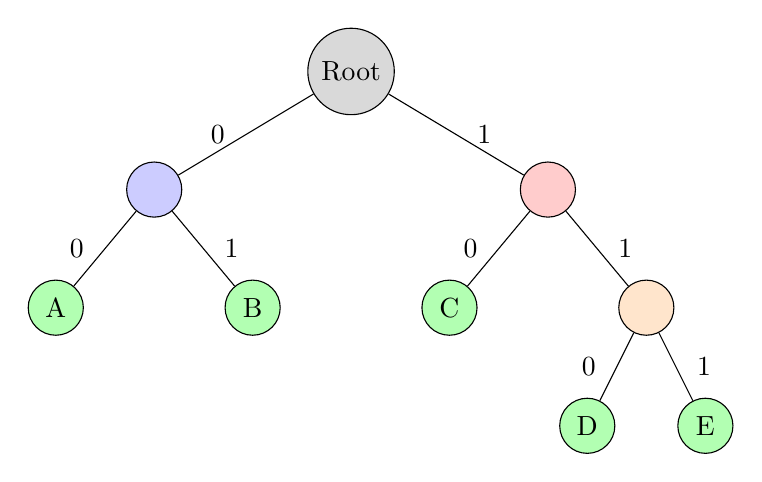
\begin{tikzpicture}[
            level distance=1.5cm,
            level 1/.style={sibling distance=5cm},
            level 2/.style={sibling distance=2.5cm},
            level 3/.style={sibling distance=1.5cm},
            every node/.style={circle,draw,minimum size=0.7cm}
        ]
            \node[fill=gray!30] {Root}
                child {
                    node[fill=blue!20] {}
                    child {
                        node[fill=green!30] {A}
                        edge from parent node[left,draw=none] {0}
                    }
                    child {
                        node[fill=green!30] {B}
                        edge from parent node[right,draw=none] {1}
                    }
                    edge from parent node[left,draw=none] {0}
                }
                child {
                    node[fill=red!20] {}
                    child {
                        node[fill=green!30] {C}
                        edge from parent node[left,draw=none] {0}
                    }
                    child {
                        node[fill=orange!20] {}
                        child {
                            node[fill=green!30] {D}
                            edge from parent node[left,draw=none] {0}
                        }
                        child {
                            node[fill=green!30] {E}
                            edge from parent node[right,draw=none] {1}
                        }
                        edge from parent node[right,draw=none] {1}
                    }
                    edge from parent node[right,draw=none] {1}
                };
        \end{tikzpicture}
    \end{center}
    
    \textbf{Decoding:} Traverse tree from root; 0=left, 1=right; leaf=output symbol
\end{frame}

%==============================================================================
\section{Shannon-Fano vs. Huffman}
%==============================================================================

\begin{frame}{Comparison with Huffman Coding}
    \begin{columns}
        \begin{column}{0.5\textwidth}
            \textbf{Shannon-Fano Coding:}
            \begin{itemize}
                \item Top-down approach
                \item Divide and assign bits
                \item Simpler to understand
                \item Not always optimal
                \item Historical importance
            \end{itemize}
        \end{column}
        \begin{column}{0.5\textwidth}
            \textbf{Huffman Coding:}
            \begin{itemize}
                \item Bottom-up approach
                \item Merge lowest probability nodes
                \item More complex construction
                \item \textbf{Always optimal}
                \item More widely used
            \end{itemize}
        \end{column}
    \end{columns}
    
    \vspace{0.5cm}
    \begin{block}{Key Difference}
        Huffman coding is \textbf{guaranteed} to produce an optimal prefix-free code, while Shannon-Fano may not achieve the absolute minimum average code length.
    \end{block}
\end{frame}

\begin{frame}{Example Where Shannon-Fano is Suboptimal}
    \textbf{Consider:} Symbols with probabilities: 0.4, 0.3, 0.2, 0.1
    
    \vspace{0.3cm}
    \begin{columns}
        \begin{column}{0.5\textwidth}
            \textbf{Shannon-Fano:}
            \begin{center}
                \begin{tabular}{c|c|c}
                    Prob & Code & Len \\
                    \midrule
                    0.4 & 0 & 1 \\
                    0.3 & 10 & 2 \\
                    0.2 & 110 & 3 \\
                    0.1 & 111 & 3 \\
                \end{tabular}
            \end{center}
            $L_{avg} = 0.4(1) + 0.3(2) + 0.2(3) + 0.1(3)$
            
            $L_{avg} = 1.9$ bits/symbol
        \end{column}
        \begin{column}{0.5\textwidth}
            \textbf{Huffman:}
            \begin{center}
                \begin{tabular}{c|c|c}
                    Prob & Code & Len \\
                    \midrule
                    0.4 & 0 & 1 \\
                    0.3 & 10 & 2 \\
                    0.2 & 110 & 3 \\
                    0.1 & 111 & 3 \\
                \end{tabular}
            \end{center}
            (Same result in this case)
            
            $L_{avg} = 1.9$ bits/symbol
        \end{column}
    \end{columns}
    
    \vspace{0.3cm}
    \textbf{Entropy:} $H = 1.846$ bits/symbol
\end{frame}

\begin{frame}{When Shannon-Fano Differs}
    \textbf{Consider:} Probabilities 0.35, 0.17, 0.17, 0.16, 0.15
    
    \vspace{0.3cm}
    \textbf{Shannon-Fano might give:}
    \begin{center}
        \begin{tabular}{c|c|c}
            Prob & SF Code & Length \\
            \midrule
            0.35 & 00 & 2 \\
            0.17 & 01 & 2 \\
            0.17 & 10 & 2 \\
            0.16 & 110 & 3 \\
            0.15 & 111 & 3 \\
        \end{tabular}
    \end{center}
    
    $L_{avg}^{SF} = 2 \times 0.69 + 3 \times 0.31 = 2.31$ bits
    
    \vspace{0.3cm}
    \textbf{Huffman achieves:} $L_{avg}^{H} = 2.30$ bits (slightly better!)
\end{frame}

%==============================================================================
\section{Applications}
%==============================================================================

\begin{frame}{Real-World Example: Image Compression}
    \textbf{How JPEG Uses Entropy Coding:}
    
    \begin{columns}
        \begin{column}{0.5\textwidth}
            \textbf{Pixel Values in a Photo:}
            \begin{itemize}
                \item Most pixels are similar to neighbors
                \item Small differences are common
                \item Large differences are rare
            \end{itemize}
            
            \vspace{0.3cm}
            \begin{center}
                \begin{tabular}{c|c}
                    \toprule
                    Difference & Frequency \\
                    \midrule
                    0 & 40\% \\
                    $\pm$1 & 25\% \\
                    $\pm$2-5 & 20\% \\
                    $>$5 & 15\% \\
                    \bottomrule
                \end{tabular}
            \end{center}
        \end{column}
        \begin{column}{0.5\textwidth}
            \textbf{Result:}
            \begin{itemize}
                \item Original photo: 10 MB
                \item After JPEG: 500 KB
                \item \textbf{95\% compression!}
            \end{itemize}
            
            \vspace{0.3cm}
            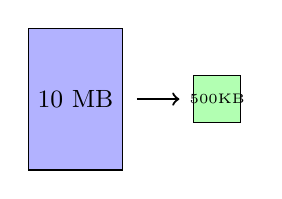
\begin{tikzpicture}[scale=0.6]
                \draw[fill=blue!30] (0,0) rectangle (2,3);
                \node at (1,1.5) {\small 10 MB};
                \draw[->,thick] (2.3,1.5) -- (3.2,1.5);
                \draw[fill=green!30] (3.5,1) rectangle (4.5,2);
                \node at (4,1.5) {\tiny 500KB};
            \end{tikzpicture}
        \end{column}
    \end{columns}
\end{frame}

\begin{frame}{Real-World Example: Text Messages}
    \textbf{SMS and Messaging Apps:}
    
    \begin{block}{Scenario}
        You type ``hello'' frequently, ``xylophone'' rarely.
    \end{block}
    
    \vspace{0.3cm}
    \begin{columns}
        \begin{column}{0.5\textwidth}
            \textbf{Without Smart Coding:}
            \begin{itemize}
                \item Each character = 8 bits
                \item ``hello'' = 40 bits
                \item ``xylophone'' = 72 bits
            \end{itemize}
        \end{column}
        \begin{column}{0.5\textwidth}
            \textbf{With Entropy Coding:}
            \begin{itemize}
                \item Common words get short codes
                \item ``hello'' $\rightarrow$ 8 bits (dictionary)
                \item Rare words = longer codes
            \end{itemize}
        \end{column}
    \end{columns}
    
    \vspace{0.5cm}
    \begin{alertblock}{Real Impact}
        WhatsApp handles 100+ billion messages/day. Even 50\% compression saves \textbf{petabytes} of bandwidth daily!
    \end{alertblock}
\end{frame}

\begin{frame}{Real-World Example: QR Codes}
    \textbf{How QR Codes Store Data Efficiently:}
    
    \begin{columns}
        \begin{column}{0.6\textwidth}
            \textbf{QR Code Modes:}
            \begin{itemize}
                \item \textbf{Numeric only:} 3.3 bits/char
                \item \textbf{Alphanumeric:} 5.5 bits/char  
                \item \textbf{Binary/Byte:} 8 bits/char
            \end{itemize}
            
            \vspace{0.3cm}
            \textbf{Why Variable Length?}
            \begin{itemize}
                \item Phone numbers: mostly digits $\rightarrow$ short codes
                \item URLs: letters + numbers $\rightarrow$ medium codes
                \item Full Unicode: all characters $\rightarrow$ longer codes
            \end{itemize}
        \end{column}
        \begin{column}{0.4\textwidth}
            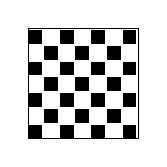
\begin{tikzpicture}[scale=0.5]
                % Simple QR-like pattern
                \foreach \x in {0,1,2,3,4,5,6} {
                    \foreach \y in {0,1,2,3,4,5,6} {
                        \pgfmathparse{mod(\x+\y,2)==0 ? "black" : "white"}
                        \fill[\pgfmathresult] (\x*0.4,\y*0.4) rectangle (\x*0.4+0.35,\y*0.4+0.35);
                    }
                }
                \draw (0,0) rectangle (2.8,2.8);
            \end{tikzpicture}
            
            \vspace{0.3cm}
            \small Same principle as Shannon-Fano!
        \end{column}
    \end{columns}
\end{frame}

\begin{frame}{Real-World Applications}
    \textbf{Shannon-Fano coding principles are used in:}
    
    \vspace{0.3cm}
    \begin{columns}
        \begin{column}{0.5\textwidth}
            \textbf{File Compression:}
            \begin{itemize}
                \item ZIP file format (historical)
                \item Early compression utilities
                \item Text file compression
            \end{itemize}
            
            \vspace{0.3cm}
            \textbf{Data Communications:}
            \begin{itemize}
                \item Fax transmission
                \item Modem protocols
                \item Network data compression
            \end{itemize}
        \end{column}
        \begin{column}{0.5\textwidth}
            \textbf{Multimedia:}
            \begin{itemize}
                \item Audio codecs
                \item Video compression
                \item Image formats
            \end{itemize}
            
            \vspace{0.3cm}
            \textbf{Modern Variants:}
            \begin{itemize}
                \item Arithmetic coding
                \item Range coding
                \item ANS (Asymmetric Numeral Systems)
            \end{itemize}
        \end{column}
    \end{columns}
\end{frame}

\begin{frame}{Compression in Practice}
    \begin{center}
        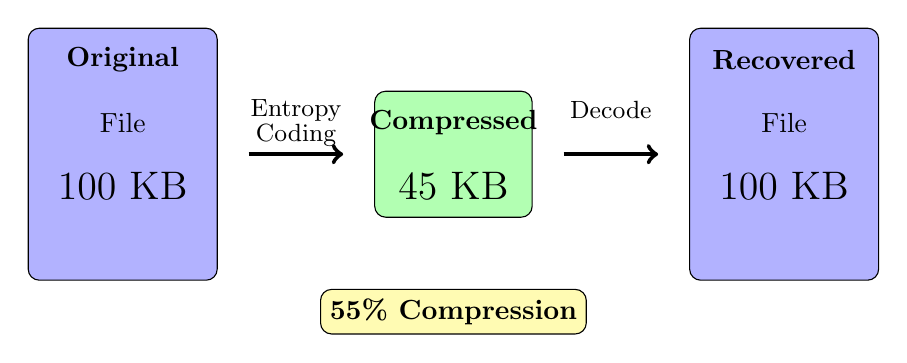
\begin{tikzpicture}[scale=0.8]
            % Original file
            \draw[fill=blue!30, rounded corners] (0,0) rectangle (3,4);
            \node at (1.5,3.5) {\textbf{Original}};
            \node at (1.5,2.5) {File};
            \node at (1.5,1.5) {\Large 100 KB};
            
            % Arrow
            \draw[->,ultra thick] (3.5,2) -- (5,2);
            \node at (4.25,2.7) {\small Entropy};
            \node at (4.25,2.3) {\small Coding};
            
            % Compressed
            \draw[fill=green!30, rounded corners] (5.5,1) rectangle (8,3);
            \node at (6.75,2.5) {\textbf{Compressed}};
            \node at (6.75,1.5) {\Large 45 KB};
            
            % Arrow
            \draw[->,ultra thick] (8.5,2) -- (10,2);
            \node at (9.25,2.7) {\small Decode};
            
            % Reconstructed
            \draw[fill=blue!30, rounded corners] (10.5,0) rectangle (13.5,4);
            \node at (12,3.5) {\textbf{Recovered}};
            \node at (12,2.5) {File};
            \node at (12,1.5) {\Large 100 KB};
            
            % Savings
            \node[draw, fill=yellow!30, rounded corners] at (6.75,-0.5) {\textbf{55\% Compression}};
        \end{tikzpicture}
    \end{center}
    
    \vspace{0.3cm}
    \textbf{Lossless compression} guarantees perfect reconstruction!
\end{frame}

%==============================================================================
\section{Practice Exercises}
%==============================================================================

%------------------------------------------------------------------------------
% Exercise 4: Image Encoding
%------------------------------------------------------------------------------
\begin{frame}{Exercise 4: Image Pattern Encoding --- Question}
    \textbf{Problem:} Analyze this 6$\times$6 pixel image and create Shannon-Fano codes.
    
    \vspace{0.5cm}
    \begin{center}
        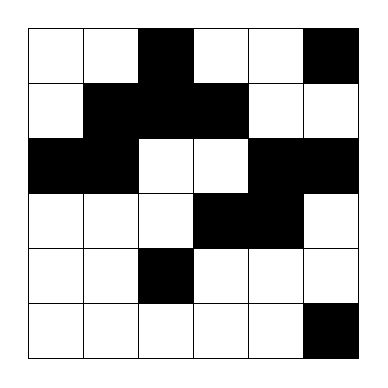
\begin{tikzpicture}[scale=0.7]
            % Row 1: W W B W W B
            \fill[white] (0,5) rectangle (1,6); \draw (0,5) rectangle (1,6);
            \fill[white] (1,5) rectangle (2,6); \draw (1,5) rectangle (2,6);
            \fill[black] (2,5) rectangle (3,6); \draw (2,5) rectangle (3,6);
            \fill[white] (3,5) rectangle (4,6); \draw (3,5) rectangle (4,6);
            \fill[white] (4,5) rectangle (5,6); \draw (4,5) rectangle (5,6);
            \fill[black] (5,5) rectangle (6,6); \draw (5,5) rectangle (6,6);
            % Row 2: W B B B W W
            \fill[white] (0,4) rectangle (1,5); \draw (0,4) rectangle (1,5);
            \fill[black] (1,4) rectangle (2,5); \draw (1,4) rectangle (2,5);
            \fill[black] (2,4) rectangle (3,5); \draw (2,4) rectangle (3,5);
            \fill[black] (3,4) rectangle (4,5); \draw (3,4) rectangle (4,5);
            \fill[white] (4,4) rectangle (5,5); \draw (4,4) rectangle (5,5);
            \fill[white] (5,4) rectangle (6,5); \draw (5,4) rectangle (6,5);
            % Row 3: B B W W B B
            \fill[black] (0,3) rectangle (1,4); \draw (0,3) rectangle (1,4);
            \fill[black] (1,3) rectangle (2,4); \draw (1,3) rectangle (2,4);
            \fill[white] (2,3) rectangle (3,4); \draw (2,3) rectangle (3,4);
            \fill[white] (3,3) rectangle (4,4); \draw (3,3) rectangle (4,4);
            \fill[black] (4,3) rectangle (5,4); \draw (4,3) rectangle (5,4);
            \fill[black] (5,3) rectangle (6,4); \draw (5,3) rectangle (6,4);
            % Row 4: W W W B B W
            \fill[white] (0,2) rectangle (1,3); \draw (0,2) rectangle (1,3);
            \fill[white] (1,2) rectangle (2,3); \draw (1,2) rectangle (2,3);
            \fill[white] (2,2) rectangle (3,3); \draw (2,2) rectangle (3,3);
            \fill[black] (3,2) rectangle (4,3); \draw (3,2) rectangle (4,3);
            \fill[black] (4,2) rectangle (5,3); \draw (4,2) rectangle (5,3);
            \fill[white] (5,2) rectangle (6,3); \draw (5,2) rectangle (6,3);
            % Row 5: W W B W W W
            \fill[white] (0,1) rectangle (1,2); \draw (0,1) rectangle (1,2);
            \fill[white] (1,1) rectangle (2,2); \draw (1,1) rectangle (2,2);
            \fill[black] (2,1) rectangle (3,2); \draw (2,1) rectangle (3,2);
            \fill[white] (3,1) rectangle (4,2); \draw (3,1) rectangle (4,2);
            \fill[white] (4,1) rectangle (5,2); \draw (4,1) rectangle (5,2);
            \fill[white] (5,1) rectangle (6,2); \draw (5,1) rectangle (6,2);
            % Row 6: W W W W W B
            \fill[white] (0,0) rectangle (1,1); \draw (0,0) rectangle (1,1);
            \fill[white] (1,0) rectangle (2,1); \draw (1,0) rectangle (2,1);
            \fill[white] (2,0) rectangle (3,1); \draw (2,0) rectangle (3,1);
            \fill[white] (3,0) rectangle (4,1); \draw (3,0) rectangle (4,1);
            \fill[white] (4,0) rectangle (5,1); \draw (4,0) rectangle (5,1);
            \fill[black] (5,0) rectangle (6,1); \draw (5,0) rectangle (6,1);
        \end{tikzpicture}
    \end{center}
    
    \vspace{0.5cm}
    \textbf{Tasks:}
    \begin{enumerate}
        \item Count Black (B) and White (W) pixels
        \item Calculate probability of each pixel value
        \item Create Shannon-Fano codes for B and W
        \item Calculate entropy and compression efficiency
    \end{enumerate}
\end{frame}

\begin{frame}{Exercise 4: Image Pattern Encoding --- Approach}
    \textbf{Step 1: Define Pixel Values}
    
    \begin{center}
        \Large W = White (0) \hspace{2cm} B = Black (1)
    \end{center}
    
    \vspace{0.3cm}
    \textbf{Step 2: Read image row by row (left to right), group in 3s for readability:}
    
    \vspace{0.3cm}
    \begin{center}
        \begin{tabular}{c|l}
            \toprule
            \textbf{Row} & \textbf{Pixel Sequence} \\
            \midrule
            Row 1 & \texttt{WWB\ \ WWB} \\
            Row 2 & \texttt{WBB\ \ BWW} \\
            Row 3 & \texttt{BBW\ \ WBB} \\
            Row 4 & \texttt{WWW\ \ BBW} \\
            Row 5 & \texttt{WWB\ \ WWW} \\
            Row 6 & \texttt{WWW\ \ WWB} \\
            \bottomrule
        \end{tabular}
    \end{center}
    
    \vspace{0.3cm}
    \textbf{Step 3: Count each symbol}
    \begin{itemize}
        \item Total pixels = $6 \times 6 = 36$
        \item Count W (White) = ?
        \item Count B (Black) = ?
    \end{itemize}
\end{frame}

\begin{frame}{Exercise 4: Solution --- Image Pattern Encoding}
    \begin{columns}
        \begin{column}{0.4\textwidth}
            \textbf{Pixel Analysis:}
            \begin{center}
                \begin{tabular}{c|c|c}
                    \toprule
                    Pixel & Count & Prob \\
                    \midrule
                    W (White) & 22 & 0.611 \\
                    B (Black) & 14 & 0.389 \\
                    \midrule
                    \textbf{Total} & \textbf{36} & \textbf{1.00} \\
                    \bottomrule
                \end{tabular}
            \end{center}
            
            \vspace{0.3cm}
            \textbf{Shannon-Fano Tree:}
            \begin{center}
                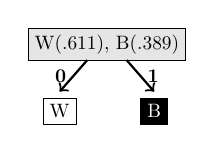
\begin{tikzpicture}[scale=0.5, every node/.style={scale=0.7}]
                    \node[draw, fill=gray!20] at (0,2) {W(.611), B(.389)};
                    \draw[->,thick] (-0.5,1.6) -- (-1.2,0.8) node[midway,left] {\textbf{0}};
                    \draw[->,thick] (0.5,1.6) -- (1.2,0.8) node[midway,right] {\textbf{1}};
                    \node[draw, fill=white] at (-1.2,0.3) {W};
                    \node[draw, fill=black, text=white] at (1.2,0.3) {B};
                \end{tikzpicture}
            \end{center}
            
            \textbf{Codes:} W = 0, B = 1
        \end{column}
        \begin{column}{0.6\textwidth}
            \textbf{Entropy:}
            \begin{align*}
                H(X) &= -(0.611 \log_2 0.611 + 0.389 \log_2 0.389) \\
                &= 0.434 + 0.530 = \boxed{0.964 \text{ bits/pixel}}
            \end{align*}
            
            \textbf{Comparison:}
            \begin{itemize}
                \item Fixed 1-bit: $36 \times 1 = 36$ bits
                \item Shannon-Fano: $36 \times 1 = 36$ bits
                \item Theoretical min: $36 \times 0.964 \approx 35$ bits
            \end{itemize}
            
            \vspace{0.2cm}
            \begin{alertblock}{Key Insight}
                With only 2 symbols, Shannon-Fano gives 1 bit each --- no compression gain over fixed encoding!
            \end{alertblock}
        \end{column}
    \end{columns}
\end{frame}

%------------------------------------------------------------------------------
% Exercise 1
%------------------------------------------------------------------------------
\begin{frame}{Exercise 1: Find Symbols and Build Shannon-Fano Code}
    \textbf{Problem:} Analyze the following data sequence and construct Shannon-Fano codes.
    
    \vspace{0.5cm}
    \begin{block}{Data Sequence (40 symbols)}
        \texttt{AAB\ AAC\ AAB\ AAA\ CAB\ AAB\ ACA\ AAB\ AAC\ ABB\ ABA\ AAB\ ACA\ A}
    \end{block}
    
    \vspace{0.5cm}
    \textbf{Tasks:}
    \begin{enumerate}
        \item Identify all unique symbols in the sequence
        \item Count the frequency of each symbol
        \item Calculate the probability of each symbol
        \item Construct the Shannon-Fano code
        \item Calculate average code length and efficiency
    \end{enumerate}
    
    \vspace{0.3cm}
    \textit{Hint: Count carefully --- there are 40 symbols total!}
\end{frame}

\begin{frame}{Exercise 1: Solution}
    \textbf{Step 1-3: Symbol Analysis}
    
    \begin{columns}
        \begin{column}{0.4\textwidth}
            \begin{center}
                \begin{tabular}{c|c|c}
                    \toprule
                    Symbol & Freq & Prob \\
                    \midrule
                    A & 24 & 0.60 \\
                    B & 10 & 0.25 \\
                    C & 6 & 0.15 \\
                    \midrule
                    \textbf{Total} & \textbf{40} & \textbf{1.00} \\
                    \bottomrule
                \end{tabular}
            \end{center}
        \end{column}
        \begin{column}{0.6\textwidth}
            \textbf{Shannon-Fano Tree:}
            \begin{center}
                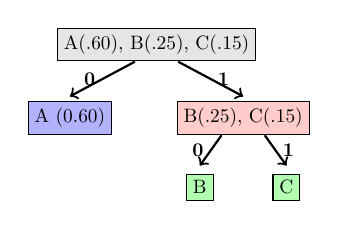
\begin{tikzpicture}[scale=0.55, every node/.style={scale=0.7}]
                    % Root
                    \node[draw, fill=gray!20] at (0,3) {A(.60), B(.25), C(.15)};
                    
                    % Level 1
                    \draw[->,thick] (-0.5,2.6) -- (-2,1.8) node[midway,left] {\textbf{0}};
                    \draw[->,thick] (0.5,2.6) -- (2,1.8) node[midway,right] {\textbf{1}};
                    
                    \node[draw, fill=blue!30] at (-2,1.3) {A (0.60)};
                    \node[draw, fill=red!20] at (2,1.3) {B(.25), C(.15)};
                    
                    % Level 2 - Right branch
                    \draw[->,thick] (1.5,0.9) -- (1,0.2) node[midway,left] {\textbf{0}};
                    \draw[->,thick] (2.5,0.9) -- (3,0.2) node[midway,right] {\textbf{1}};
                    
                    \node[draw, fill=green!30] at (1,-0.3) {B};
                    \node[draw, fill=green!30] at (3,-0.3) {C};
                \end{tikzpicture}
            \end{center}
        \end{column}
    \end{columns}
    
    \vspace{0.2cm}
    \textbf{Final Codes:} A = 0, B = 10, C = 11
\end{frame}

\begin{frame}{Exercise 1: Solution (Continued)}
    \textbf{Final Codes:}
    \begin{center}
        \begin{tabular}{c|c|c|c|c}
            \toprule
            Symbol & Probability & Code & Length & $p_i \times l_i$ \\
            \midrule
            A & 0.60 & 0 & 1 & 0.60 \\
            B & 0.25 & 10 & 2 & 0.50 \\
            C & 0.15 & 11 & 2 & 0.30 \\
            \midrule
            \multicolumn{4}{r|}{\textbf{Average Code Length $L_{avg}$:}} & \textbf{1.40} \\
            \bottomrule
        \end{tabular}
    \end{center}
    
    \vspace{0.3cm}
    \textbf{Performance Analysis:}
    \begin{align*}
        H(X) &= -(0.60 \log_2 0.60 + 0.25 \log_2 0.25 + 0.15 \log_2 0.15) \\
        &= -(0.60 \times (-0.737) + 0.25 \times (-2) + 0.15 \times (-2.737)) \\
        &= 0.442 + 0.500 + 0.411 = \boxed{1.353 \text{ bits/symbol}}
    \end{align*}
    
    \textbf{Efficiency:} $\eta = \frac{1.353}{1.40} \times 100\% = \boxed{96.64\%}$
    
    \textbf{Redundancy:} $R = 1.40 - 1.353 = \boxed{0.047 \text{ bits/symbol}}$
\end{frame}

%------------------------------------------------------------------------------
% Exercise 2
%------------------------------------------------------------------------------
\begin{frame}{Exercise 2: Find Symbols and Build Shannon-Fano Code}
    \textbf{Problem:} Analyze the following message sequence and construct Shannon-Fano codes.
    
    \vspace{0.5cm}
    \begin{block}{Message Sequence (50 symbols)}
        \texttt{SUN\ MON\ SUN\ TUE\ SUN\ WED\ SUN\ MON\ SUN\ THU\ SUN\ MON\ FRI\ SUN\ MON\ SAT\ SUN}
    \end{block}
    
    \vspace{0.5cm}
    \textbf{Tasks:}
    \begin{enumerate}
        \item Identify all unique symbols (day codes)
        \item Count the frequency of each symbol
        \item Calculate the probability of each symbol
        \item Construct the Shannon-Fano code
        \item Calculate average code length, entropy, and efficiency
    \end{enumerate}
    
    \vspace{0.3cm}
    \textit{Hint: This represents weekly schedule data --- some days appear more often!}
\end{frame}

\begin{frame}{Exercise 2: Solution}
    \textbf{Step 1-3: Symbol Analysis} (Sorted by probability)
    
    \begin{center}
        \begin{tabular}{c|c|c}
            \toprule
            Symbol & Frequency & Probability \\
            \midrule
            SUN & 9 & 0.36 \\
            MON & 4 & 0.16 \\
            TUE & 1 & 0.04 \\
            WED & 1 & 0.04 \\
            THU & 1 & 0.04 \\
            FRI & 1 & 0.04 \\
            SAT & 1 & 0.04 \\
            \midrule
            \textbf{Total} & \textbf{18} & --- \\
            \bottomrule
        \end{tabular}
    \end{center}
    
    \vspace{0.2cm}
    \textit{Note: Counting 3-letter day codes as symbols. Each space-separated group = 1 symbol.}
    
    \textbf{Corrected probabilities:} SUN=9/18=0.50, MON=4/18=0.222, others=1/18=0.056 each
\end{frame}

\begin{frame}{Exercise 2: Solution --- Shannon-Fano Tree}
    \begin{center}
        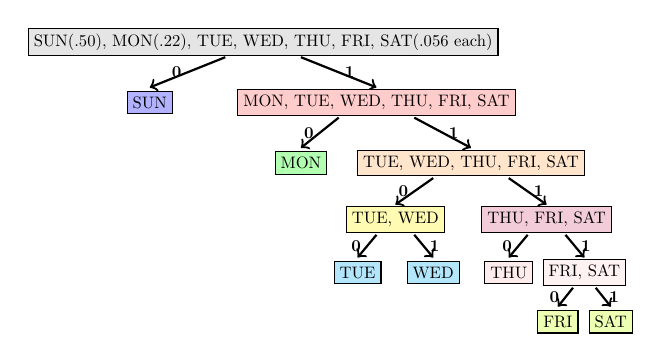
\begin{tikzpicture}[scale=0.48, every node/.style={scale=0.6}]
            % Level 0
            \node[draw, fill=gray!20] at (0,4) {SUN(.50), MON(.22), TUE, WED, THU, FRI, SAT(.056 each)};
            
            % Level 1
            \draw[->,thick] (-1,3.6) -- (-3,2.8) node[midway,left] {\textbf{0}};
            \draw[->,thick] (1,3.6) -- (3,2.8) node[midway,right] {\textbf{1}};
            
            \node[draw, fill=blue!30] at (-3,2.4) {SUN};
            \node[draw, fill=red!20] at (3,2.4) {MON, TUE, WED, THU, FRI, SAT};
            
            % Level 2 - Right
            \draw[->,thick] (2,2) -- (1,1.2) node[midway,left] {\textbf{0}};
            \draw[->,thick] (4,2) -- (5.5,1.2) node[midway,right] {\textbf{1}};
            
            \node[draw, fill=green!30] at (1,0.8) {MON};
            \node[draw, fill=orange!20] at (5.5,0.8) {TUE, WED, THU, FRI, SAT};
            
            % Level 3
            \draw[->,thick] (4.5,0.4) -- (3.5,-0.3) node[midway,left] {\textbf{0}};
            \draw[->,thick] (6.5,0.4) -- (7.5,-0.3) node[midway,right] {\textbf{1}};
            
            \node[draw, fill=yellow!30] at (3.5,-0.7) {TUE, WED};
            \node[draw, fill=purple!20] at (7.5,-0.7) {THU, FRI, SAT};
            
            % Level 4 Left
            \draw[->,thick] (3,-1.1) -- (2.5,-1.7) node[midway,left] {\textbf{0}};
            \draw[->,thick] (4,-1.1) -- (4.5,-1.7) node[midway,right] {\textbf{1}};
            \node[draw, fill=cyan!30] at (2.5,-2.1) {TUE};
            \node[draw, fill=cyan!30] at (4.5,-2.1) {WED};
            
            % Level 4 Right
            \draw[->,thick] (7,-1.1) -- (6.5,-1.7) node[midway,left] {\textbf{0}};
            \draw[->,thick] (8,-1.1) -- (8.5,-1.7) node[midway,right] {\textbf{1}};
            \node[draw, fill=pink!30] at (6.5,-2.1) {THU};
            \node[draw, fill=pink!20] at (8.5,-2.1) {FRI, SAT};
            
            % Level 5
            \draw[->,thick] (8.2,-2.5) -- (7.8,-3) node[midway,left] {\textbf{0}};
            \draw[->,thick] (8.8,-2.5) -- (9.2,-3) node[midway,right] {\textbf{1}};
            \node[draw, fill=lime!30] at (7.8,-3.4) {FRI};
            \node[draw, fill=lime!30] at (9.2,-3.4) {SAT};
        \end{tikzpicture}
    \end{center}
    
    \vspace{0.1cm}
    \small\textbf{Codes:} SUN=0, MON=10, TUE=1100, WED=1101, THU=1110, FRI=11110, SAT=11111
\end{frame}

\begin{frame}{Exercise 2: Solution --- Final Codes and Analysis}
    \textbf{Final Shannon-Fano Codes:}
    \begin{center}
        \begin{tabular}{c|c|c|c|c}
            \toprule
            Symbol & Probability & Code & Length & $p_i \times l_i$ \\
            \midrule
            SUN & 0.500 & 0 & 1 & 0.500 \\
            MON & 0.222 & 10 & 2 & 0.444 \\
            TUE & 0.056 & 1100 & 4 & 0.224 \\
            WED & 0.056 & 1101 & 4 & 0.224 \\
            THU & 0.056 & 1110 & 4 & 0.224 \\
            FRI & 0.056 & 11110 & 5 & 0.280 \\
            SAT & 0.056 & 11111 & 5 & 0.280 \\
            \midrule
            \multicolumn{4}{r|}{\textbf{Average Code Length $L_{avg}$:}} & \textbf{2.176} \\
            \bottomrule
        \end{tabular}
    \end{center}
    
    \vspace{0.2cm}
    \textbf{Entropy:} $H(X) = 2.055$ bits/symbol
    
    \textbf{Efficiency:} $\eta = \frac{2.055}{2.176} \times 100\% = \boxed{94.44\%}$
    
    \textbf{Redundancy:} $R = 2.176 - 2.055 = \boxed{0.121 \text{ bits/symbol}}$
\end{frame}

%------------------------------------------------------------------------------
% Exercise 3
%------------------------------------------------------------------------------
\begin{frame}{Exercise 3: Find Symbols and Build Shannon-Fano Code}
    \textbf{Problem:} A sensor transmits the following readings. Construct Shannon-Fano codes.
    
    \vspace{0.5cm}
    \begin{block}{Sensor Data Sequence (60 readings)}
        \texttt{LOW\ LOW\ MED\ LOW\ HIG\ LOW\ LOW\ MED\ LOW\ LOW\ CRI\ LOW\ MED\ LOW\ LOW\ LOW\ MED\ HIG\ LOW\ LOW}
    \end{block}
    
    \vspace{0.5cm}
    \textbf{Tasks:}
    \begin{enumerate}
        \item Identify all unique sensor states
        \item Count the frequency of each state
        \item Calculate the probability of each state
        \item Construct the Shannon-Fano code
        \item Calculate average code length, entropy, and efficiency
        \item Encode the message: ``MED LOW CRI HIG''
    \end{enumerate}
    
    \vspace{0.3cm}
    \textit{Hint: States are LOW (normal), MED (medium), HIG (high alert), CRI (critical)}
\end{frame}

\begin{frame}{Exercise 3: Solution}
    \textbf{Symbol Analysis} (Sorted by probability)
    
    \begin{columns}
        \begin{column}{0.35\textwidth}
            \begin{center}
                \small
                \begin{tabular}{c|c|c}
                    \toprule
                    Symbol & Freq & Prob \\
                    \midrule
                    LOW & 13 & 0.65 \\
                    MED & 4 & 0.20 \\
                    HIG & 2 & 0.10 \\
                    CRI & 1 & 0.05 \\
                    \midrule
                    \textbf{Total} & \textbf{20} & \textbf{1.00} \\
                    \bottomrule
                \end{tabular}
            \end{center}
        \end{column}
        \begin{column}{0.65\textwidth}
            \textbf{Shannon-Fano Tree:}
            \begin{center}
                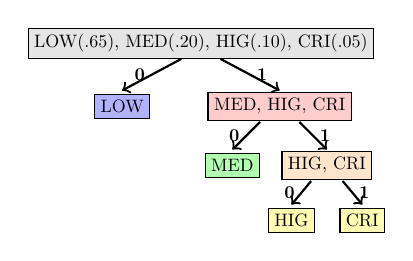
\begin{tikzpicture}[scale=0.5, every node/.style={scale=0.65}]
                    % Level 0
                    \node[draw, fill=gray!20] at (0,3.5) {LOW(.65), MED(.20), HIG(.10), CRI(.05)};
                    
                    % Level 1
                    \draw[->,thick] (-0.5,3.1) -- (-2,2.3) node[midway,left] {\textbf{0}};
                    \draw[->,thick] (0.5,3.1) -- (2,2.3) node[midway,right] {\textbf{1}};
                    
                    \node[draw, fill=blue!30] at (-2,1.9) {LOW};
                    \node[draw, fill=red!20] at (2,1.9) {MED, HIG, CRI};
                    
                    % Level 2 - Right
                    \draw[->,thick] (1.5,1.5) -- (0.8,0.8) node[midway,left] {\textbf{0}};
                    \draw[->,thick] (2.5,1.5) -- (3.2,0.8) node[midway,right] {\textbf{1}};
                    
                    \node[draw, fill=green!30] at (0.8,0.4) {MED};
                    \node[draw, fill=orange!20] at (3.2,0.4) {HIG, CRI};
                    
                    % Level 3
                    \draw[->,thick] (2.8,0) -- (2.3,-0.6) node[midway,left] {\textbf{0}};
                    \draw[->,thick] (3.6,0) -- (4.1,-0.6) node[midway,right] {\textbf{1}};
                    
                    \node[draw, fill=yellow!30] at (2.3,-1) {HIG};
                    \node[draw, fill=yellow!30] at (4.1,-1) {CRI};
                \end{tikzpicture}
            \end{center}
        \end{column}
    \end{columns}
    
    \vspace{0.2cm}
    \textbf{Final Codes:} LOW = 0, MED = 10, HIG = 110, CRI = 111
\end{frame}

\begin{frame}{Exercise 3: Solution --- Final Codes and Analysis}
    \textbf{Final Shannon-Fano Codes:}
    \begin{center}
        \begin{tabular}{c|c|c|c|c}
            \toprule
            Symbol & Probability & Code & Length & $p_i \times l_i$ \\
            \midrule
            LOW & 0.65 & 0 & 1 & 0.65 \\
            MED & 0.20 & 10 & 2 & 0.40 \\
            HIG & 0.10 & 110 & 3 & 0.30 \\
            CRI & 0.05 & 111 & 3 & 0.15 \\
            \midrule
            \multicolumn{4}{r|}{\textbf{Average Code Length $L_{avg}$:}} & \textbf{1.50} \\
            \bottomrule
        \end{tabular}
    \end{center}
    
    \vspace{0.3cm}
    \textbf{Entropy:} $H(X) = -(0.65 \log_2 0.65 + 0.20 \log_2 0.20 + 0.10 \log_2 0.10 + 0.05 \log_2 0.05)$
    \begin{equation*}
        H(X) = 0.406 + 0.464 + 0.332 + 0.216 = \boxed{1.418 \text{ bits/symbol}}
    \end{equation*}
    
    \textbf{Efficiency:} $\eta = \frac{1.418}{1.50} \times 100\% = \boxed{94.53\%}$
    
    \vspace{0.2cm}
    \textbf{Encoding ``MED LOW CRI HIG'':} $10 + 0 + 111 + 110 = \boxed{100111110}$ (9 bits)
\end{frame}

%==============================================================================
\section{Summary}
%==============================================================================

\begin{frame}{Key Takeaways}
    \begin{enumerate}
        \item \textbf{Entropy} measures the average information content
        \begin{equation*}
            H(X) = -\sum_{i} p_i \log_2 p_i
        \end{equation*}
        
        \item \textbf{Shannon-Fano} is a prefix-free, variable-length coding technique
        
        \item \textbf{Algorithm:} Sort $\rightarrow$ Divide equally $\rightarrow$ Assign 0/1 $\rightarrow$ Recurse
        
        \item \textbf{Average code length} should satisfy:
        \begin{equation*}
            H(X) \leq L_{avg} < H(X) + 1
        \end{equation*}
        
        \item \textbf{Efficiency:} $\eta = \frac{H(X)}{L_{avg}} \times 100\%$
        
        \item Shannon-Fano is \textbf{near-optimal} but \textbf{not always optimal}
    \end{enumerate}
\end{frame}

\begin{frame}{Practice Problems}
    \textbf{Problem 1:} Construct Shannon-Fano codes for:
    \begin{center}
        \begin{tabular}{c|ccccc}
            Symbol & A & B & C & D & E \\
            \midrule
            Probability & 0.40 & 0.20 & 0.15 & 0.15 & 0.10 \\
        \end{tabular}
    \end{center}
    
    \vspace{0.3cm}
    \textbf{Problem 2:} Given these codes, verify they are prefix-free:
    \begin{center}
        A=0, B=10, C=110, D=1110, E=1111
    \end{center}
    
    \vspace{0.3cm}
    \textbf{Problem 3:} A source has entropy 2.5 bits/symbol. A code achieves $L_{avg} = 2.7$ bits/symbol. Calculate efficiency and redundancy.
    
    \vspace{0.3cm}
    \textbf{Problem 4:} Encode ``CABBAGE'' using the code from Problem 1.
\end{frame}

\begin{frame}{Important Formulas Summary}
    \begin{block}{Entropy}
        $H(X) = -\sum_{i=1}^{n} p_i \log_2 p_i$
    \end{block}
    
    \begin{block}{Average Code Length}
        $L_{avg} = \sum_{i=1}^{n} p_i \cdot l_i$
    \end{block}
    
    \begin{block}{Efficiency}
        $\eta = \frac{H(X)}{L_{avg}} \times 100\%$
    \end{block}
    
    \begin{block}{Redundancy}
        $R = L_{avg} - H(X)$
    \end{block}
\end{frame}

\begin{frame}
    \begin{center}
        \Huge{\textbf{Thank You!}}
        
        \vspace{1cm}
        \Large{Questions?}
        
        \vspace{1.5cm}
        \normalsize
        \textit{``The fundamental problem of communication is that of reproducing at one point either exactly or approximately a message selected at another point.''}
        
        \vspace{0.3cm}
        --- Claude Shannon, 1948
    \end{center}
\end{frame}

\end{document}
